% =============================================
% LOF & centroid 補足説明追加版
% =============================================

\documentclass[a4j,dvipdfmx]{jsarticle}
\usepackage{graphicx}
\usepackage{amsmath}
\usepackage{url}
\usepackage{algorithm}
\usepackage{algorithmic}
\usepackage{booktabs}
\usepackage{float} % 図の位置制御用

\floatname{algorithm}{アルゴリズム}

% 浮動体のパラメータ調整
\renewcommand{\topfraction}{0.85}
\renewcommand{\bottomfraction}{0.85}
\renewcommand{\textfraction}{0.15}
\renewcommand{\floatpagefraction}{0.7}

\title{二次元データに対する k-means クラスタリングと Local Outlier Factor の C\# 実装}
\author{大阪大学 工学部 電子情報学科 3 年\\情報システム工学コース\\08D23091\,辻\,孝弥}
\date{\today}

%--------------------------------------------------
\begin{document}
\maketitle
\tableofcontents
\newpage

%--------------------------------------------------
\begin{abstract}
CSV 形式で与えられた最大 200 点の二次元データに対し,Local Outlier Factor (LOF) による外れ値検出と k-means クラスタリングを単一の C\# プログラムで逐次実行した手順と結果を報告する.本稿では実装の要点,入力・出力仕様,および実験ログの要約を整理し,将来の改善方針を示す.
\end{abstract}

%--------------------------------------------------
\section{背景と目的}
外れ値検出とクラスタリングはデータ解析の根幹であり,両者は相互に影響を及ぼす.本プログラムは LOF によって外れ値を除いた後に k-means を適用することで,クラスタリング結果の安定化を図ることを目的としている.

%--------------------------------------------------
\section{手法}
\subsection{処理フロー}
\begin{description}
  \item[入力] 二次元座標を格納した CSV(形式:\texttt{x,y})
  \item[処理手順]
    \begin{enumerate}
      \item CSV 読み込み
      \item LOF の計算 ($k=10$)
      \item 閾値 1.2 を超える点を外れ値とフラグ付け
      \item k-means クラスタリング(クラスタ数 $k$ はコマンドライン引数,既定値 3)
      \item 結果を CSV へ出力
    \end{enumerate}
  \item[出力] \texttt{x, y, cluster\_id, is\_outlier}
\end{description}

\subsection{Local Outlier Factor (LOF)}
スクリーンショットで示された定義に合わせ,点 $A$ の LOF は次式で与えられる:
\begin{equation}
  \operatorname{LOF}_k(A)
  :=
  \frac{\displaystyle\sum_{B\in N_k(A)} \operatorname{lrd}_k(B) \,/\, |N_k(A)|}
       {\operatorname{lrd}_k(A)}\,.
  \label{eq:lof}
\end{equation}
ここで $N_k(A)$ は $A$ の $k$ 近傍集合,$|N_k(A)|=k$,$\operatorname{lrd}_k(\cdot)$ は局所到達可能密度 (Local Reachability Density) である。

\subsection{k-means クラスタリング}
初期重心はランダムに抽出し,ユークリッド距離による割り当てと重心再計算を繰り返す.収束判定は
\[
  \max_{j} \bigl\| \mathbf{c}_{j}^{(t+1)} - \mathbf{c}_{j}^{(t)} \bigr\| < 10^{-8}
\]
または 1000 反復に達した時点とした.ここで $\mathbf{c}_{j}^{(t)}$ は時刻 $t$ におけるクラスタ $j$ の重心 (centroid) であり,プログラム中の変数 \texttt{centroid[j, *]} に対応する。外れ値は重心計算から除外する.

%--------------------------------------------------
\section{実装要点 (C\#)}
\begin{itemize}
  \item 2 次元データは \texttt{double[,]} 配列で保持.最大 200 行を想定.
  \item LOF 計算と k-means は同一ファイルで実装し,外部依存ライブラリは使用していない.
  \item 外れ値を除外して重心を計算する際のコード片をアルゴリズム~\ref{lst:centroid} に示す.
\end{itemize}

\begin{algorithm}[tbp]
\caption{外れ値除外付き重心計算 (抜粋)}
\label{lst:centroid}
\begin{algorithmic}[1]
\FOR{$i \gets 0$ \TO $N-1$}
  \IF{$label[i]==k$ \AND $is\_outlier[i]==\text{false}$}
    \STATE $\text{sum}_x \mathrel{+}= data[i,0]$;
    \STATE $\text{sum}_y \mathrel{+}= data[i,1]$;
    \STATE $\text{count} \mathrel{+}=1$;
  \ENDIF
\ENDFOR
\end{algorithmic}
\end{algorithm}

%--------------------------------------------------
\section{実験設定}
\subsection{データセット}
5 種の人工データ (各 200 点) を使用した:moon,crater,square,three\_island,two\_island.

\subsection{パラメータ}
LOF は $k=10$,閾値 1.2,k-means はクラスタ数 $k=3$ とし,最大 1000 反復で収束を判定した.

%--------------------------------------------------
\section{結果}
\subsection{外れ値検出結果 (moon データセット)}
式~\eqref{eq:lof} に従い計算した LOF が 1.2 を超えた点は 7 個であり,表~\ref{tab:outliers} に示す.

\begin{table}[tbp]
  \centering
  \caption{外れ値一覧 (LOF $>1.2$)}
  \label{tab:outliers}
  \begin{tabular}{ccc}
    \toprule
    No. & 座標 $(x,y)$ & LOF 値 \\
    \midrule
    1 & (0.2082, 0.9957) & 1.3159 \\
    2 & (0.1641, 1.0172) & 1.2992 \\
    3 & (0.3043, 1.0289) & 1.2795 \\
    4 & (2.2251, 0.9604) & 1.2248 \\
    5 & (0.2126, 0.9937) & 1.3193 \\
    6 & (3.1527, 1.5360) & 1.2000 \\
    7 & (1.1774, 1.6019) & 1.2411 \\
    \bottomrule
  \end{tabular}
\end{table}
\subsection{k-means 収束状況}
初期重心をランダムに選択した場合,moon データセットでは 13 反復で収束した.各反復で外れ値 7 点は重心計算から除外された.

\subsection{可視化結果}
\begin{figure}[H] % H オプションで厳密に位置を固定
  \centering
  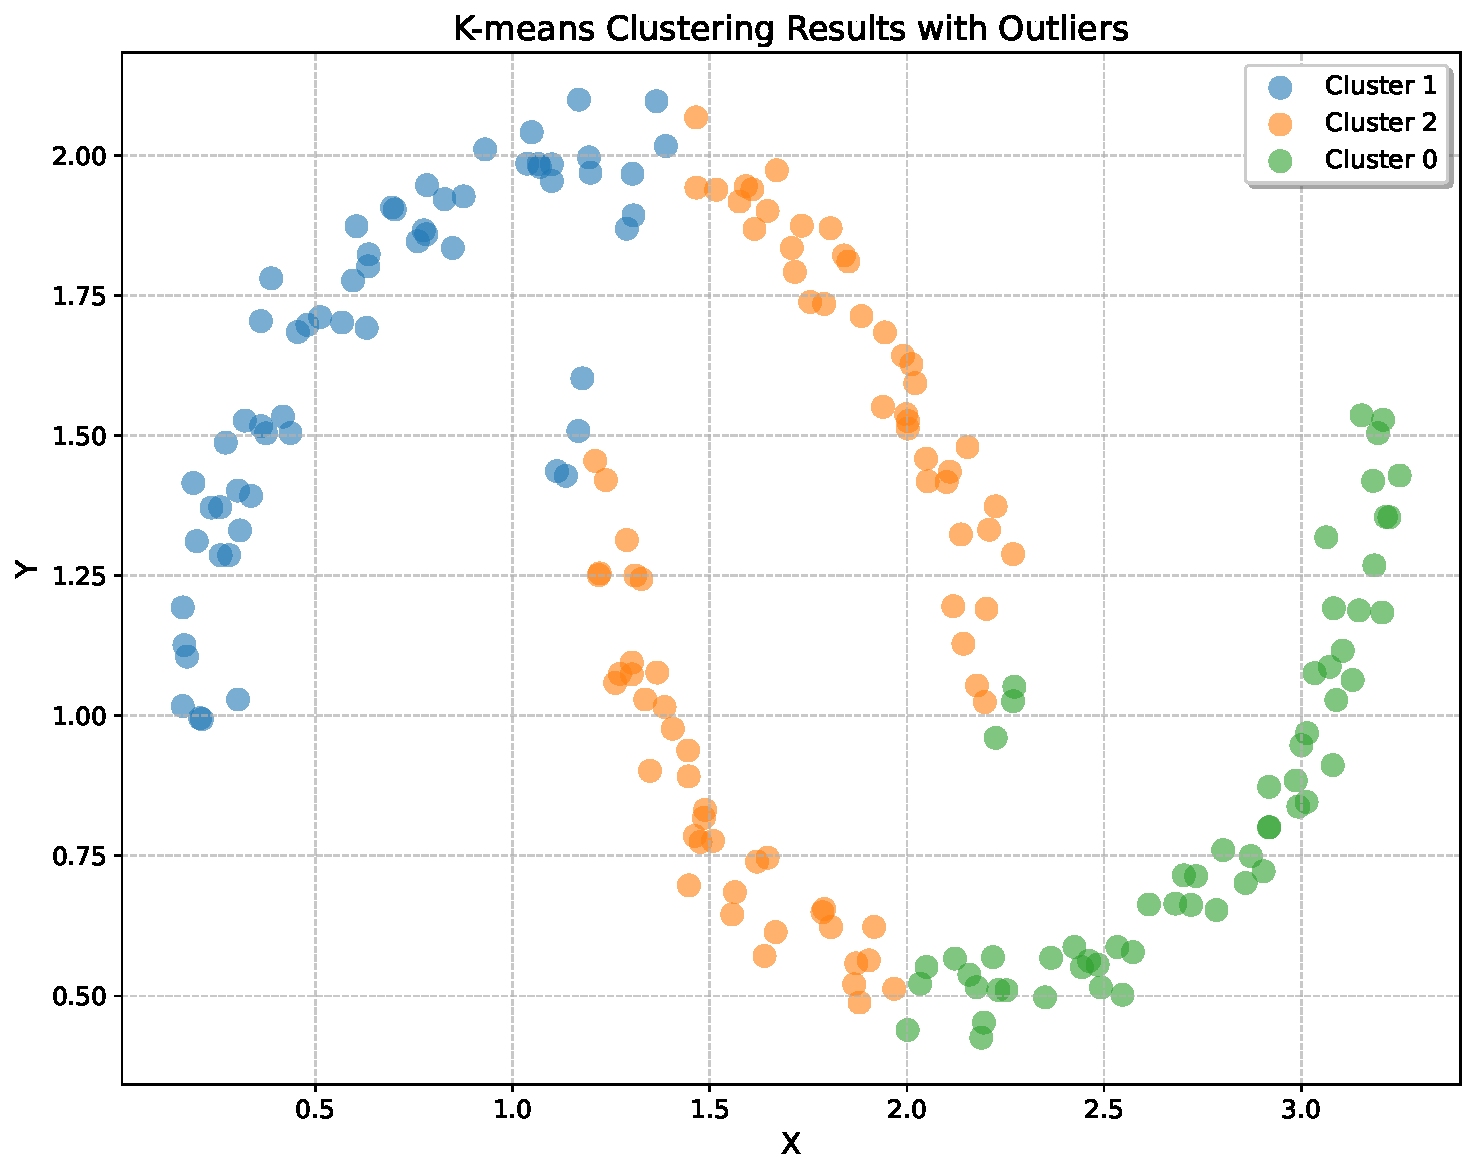
\includegraphics[width=.4\textwidth]{moon_output_plot.pdf}
  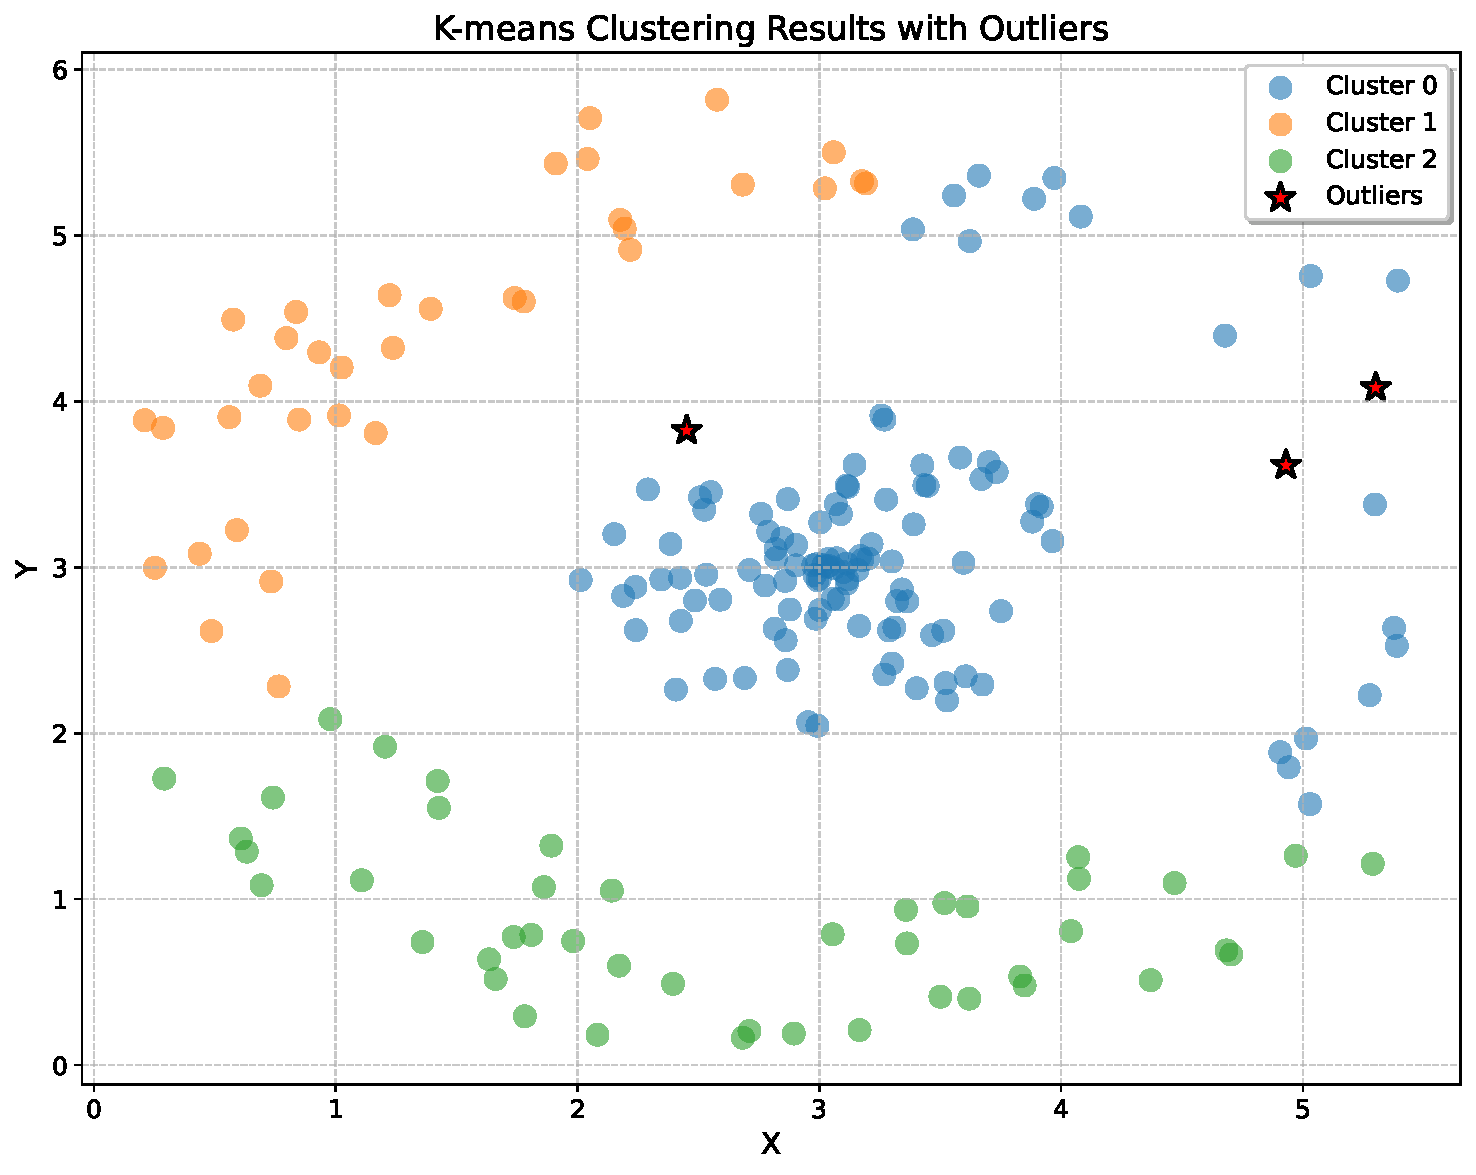
\includegraphics[width=.4\textwidth]{crater_output_plot.pdf}
  \caption{moon(左)と crater(右)のクラスタリング結果}
  \label{fig:moon-crater}
\end{figure}

\begin{figure}[H] % H オプションで厳密に位置を固定
  \centering
  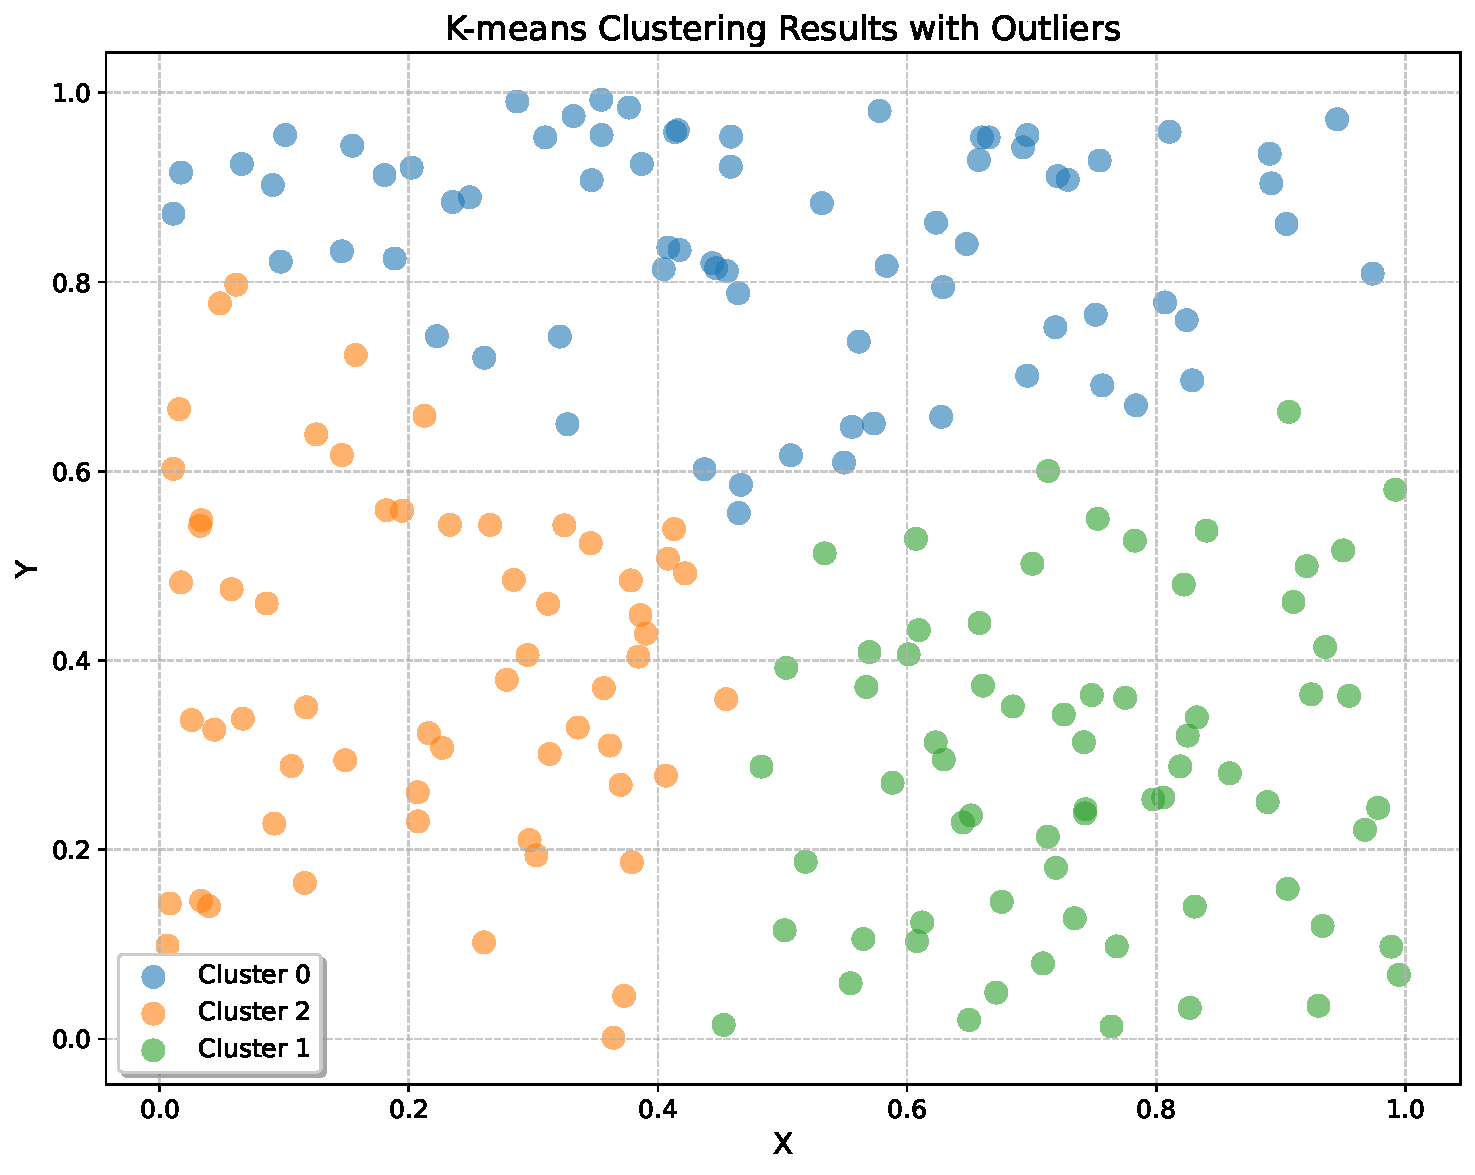
\includegraphics[width=.4\textwidth]{square_output_plot.pdf}
  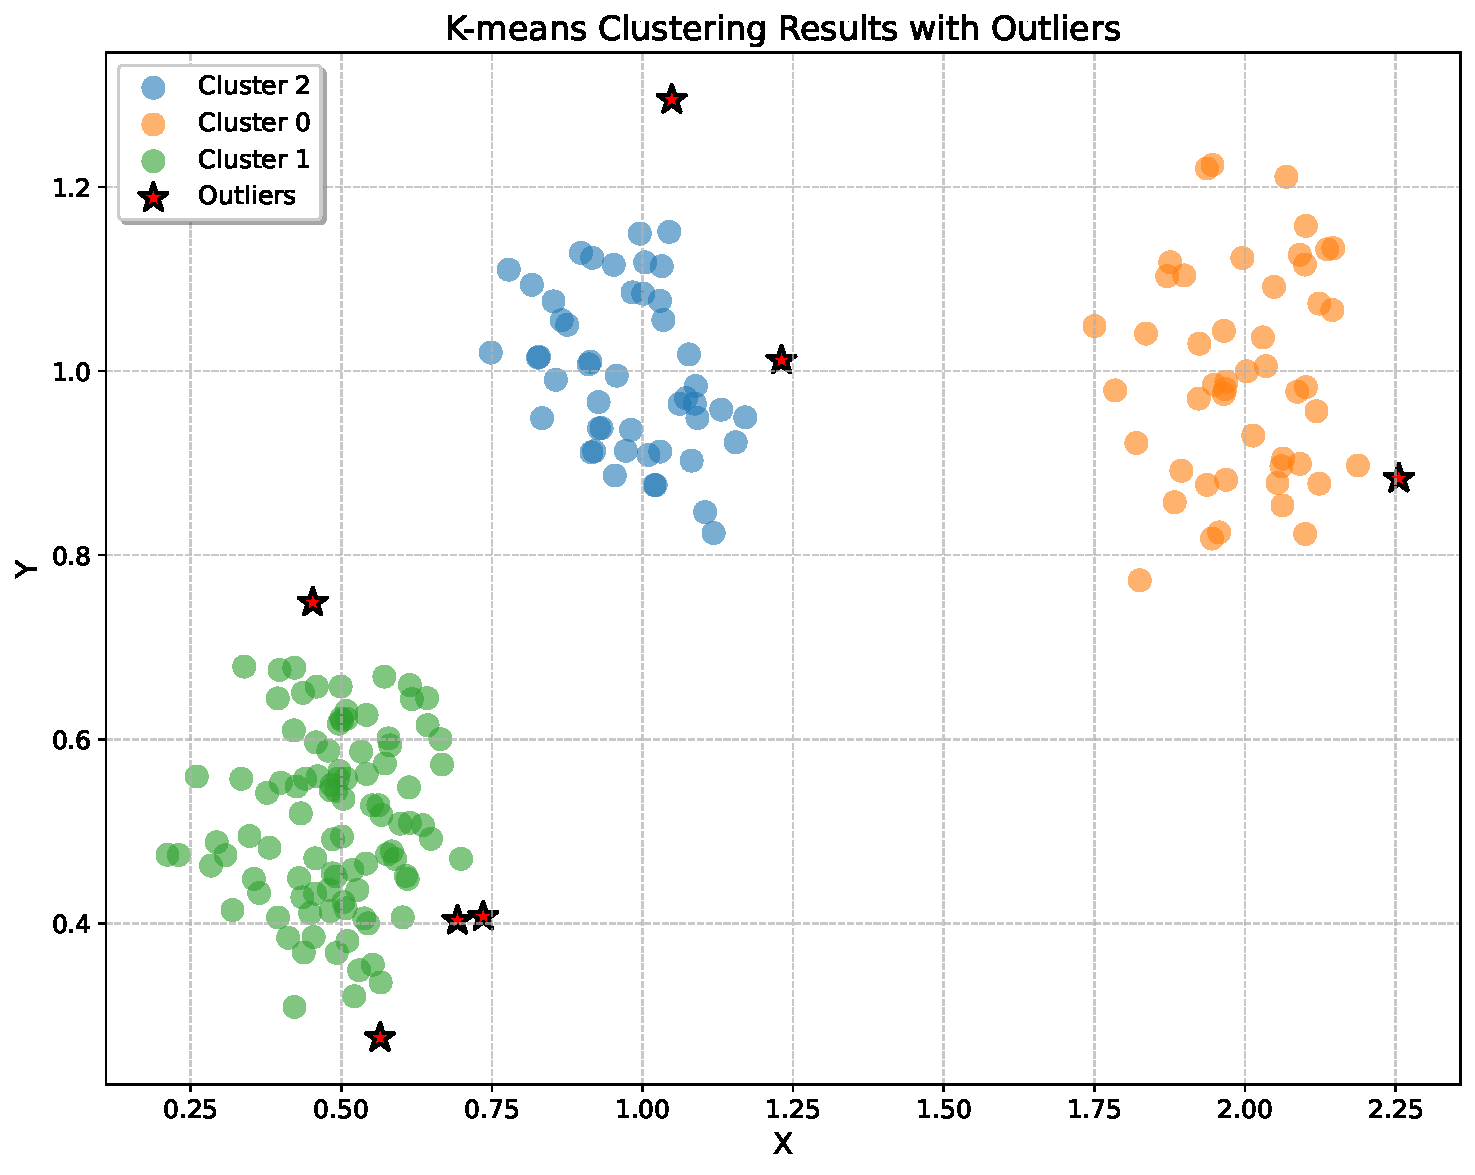
\includegraphics[width=.4\textwidth]{three_island_output_plot.pdf}
  \caption{square(左)と three\_island(右)のクラスタリング結果}
  \label{fig:square-three}
\end{figure}

\begin{figure}[H] % H オプションで厳密に位置を固定
  \centering
  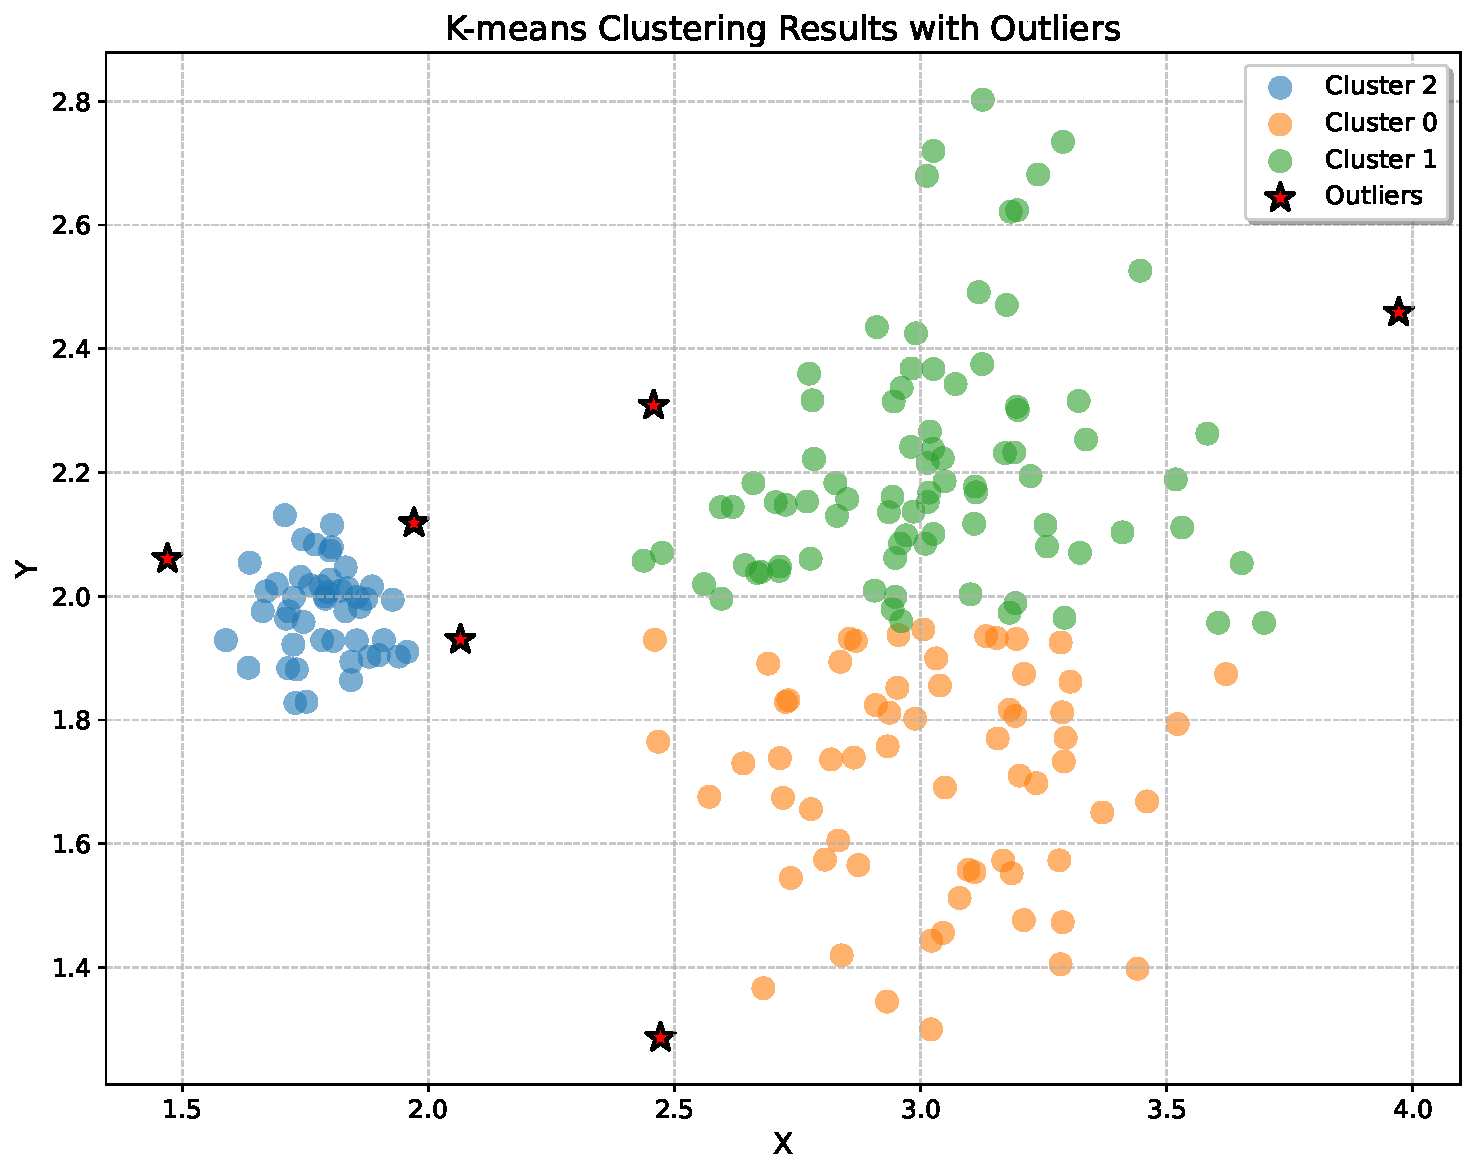
\includegraphics[width=.4\textwidth]{two_island_output_plot.pdf}
  \caption{two\_island データセットのクラスタリング結果}
  \label{fig:two-island}
\end{figure}

%--------------------------------------------------
\section{考察}
\begin{enumerate}
  \item 式~\eqref{eq:lof} に基づき外れ値を除外しながら計算した重心 $\mathbf{c}_j$ により,クラスタリングの安定性が向上した。
  \item moon データセットのような非線形境界に対しては k-means の線形判別面が不利であり,今後は DBSCAN などの導入を検討する必要がある。
\end{enumerate}

%--------------------------------------------------
\section{まとめ}
本稿で示した C\# プログラムは,LOF による外れ値検出と k-means クラスタリングを連続実行し,200 点のデータに対して 13 反復で収束したことを確認した。外れ値除去付き重心計算(変数 	exttt{centroid[j,*]} が対応)がクラスタ分割の安定化に寄与することを示した。

今後は LOF 閾値の最適化,自動初期化手法(k-means++),および非線形クラスタリング手法の比較実装を課題とする。

\end{document}
